%----------------------------------------------------------------------------------------
%	PROBLEM 1
%----------------------------------------------------------------------------------------

% To have just one problem per page, simply put a \clearpage after each problem
\newpage
\begin{homeworkProblem}
\section{Iterative improvement algorithms}
\subsection{Problem statement}
Implement iterative improvement algorithms with:
\begin{itemize}
  \item first-improvement
  \item best-improvement
\end{itemize}
pivoting rule for each of the three neighborhoods: transpose, exchange, and insert. \\
As a starting solution for iterative improvement, consider a random permutation, that is, use the method “Uninformed Random Picking” (see slides of lectures). Bonus points will be awarded for also considering an insertion heuristic as an alternative to random initialization.
\begin{enumerate}
  \item Run the 6 resulting iterative improvement algorithms (all combinations of the two pivoting rules and the
three neighborhoods) on each of the instances. Repeat each run 100 times with different seed for the random
number generator.
\item Compute the following statistics for each of the 6 iterative improvement algorithms and each instance:
\begin{itemize}
  \item Percentage of runs with constraint violations
  \item Mean penalised relative percentage deviation
  \item Mean computation time
\end{itemize} 
\item Produce boxplots of penalised relative percentage deviation and computation time per instance.
\item Determine using statistical tests (in this case, the Wilcoxon test), whether there is a statistically significant difference between the quality of the solutions generated by the different algorithms.
In particular, compare best vs. first-improvement for each neighborhood, and exchange vs. insertion for each pivoting rule.
\end{enumerate}

\subsection{Experiment results}
\subsubsection{n80w20.001}
\begin{center}
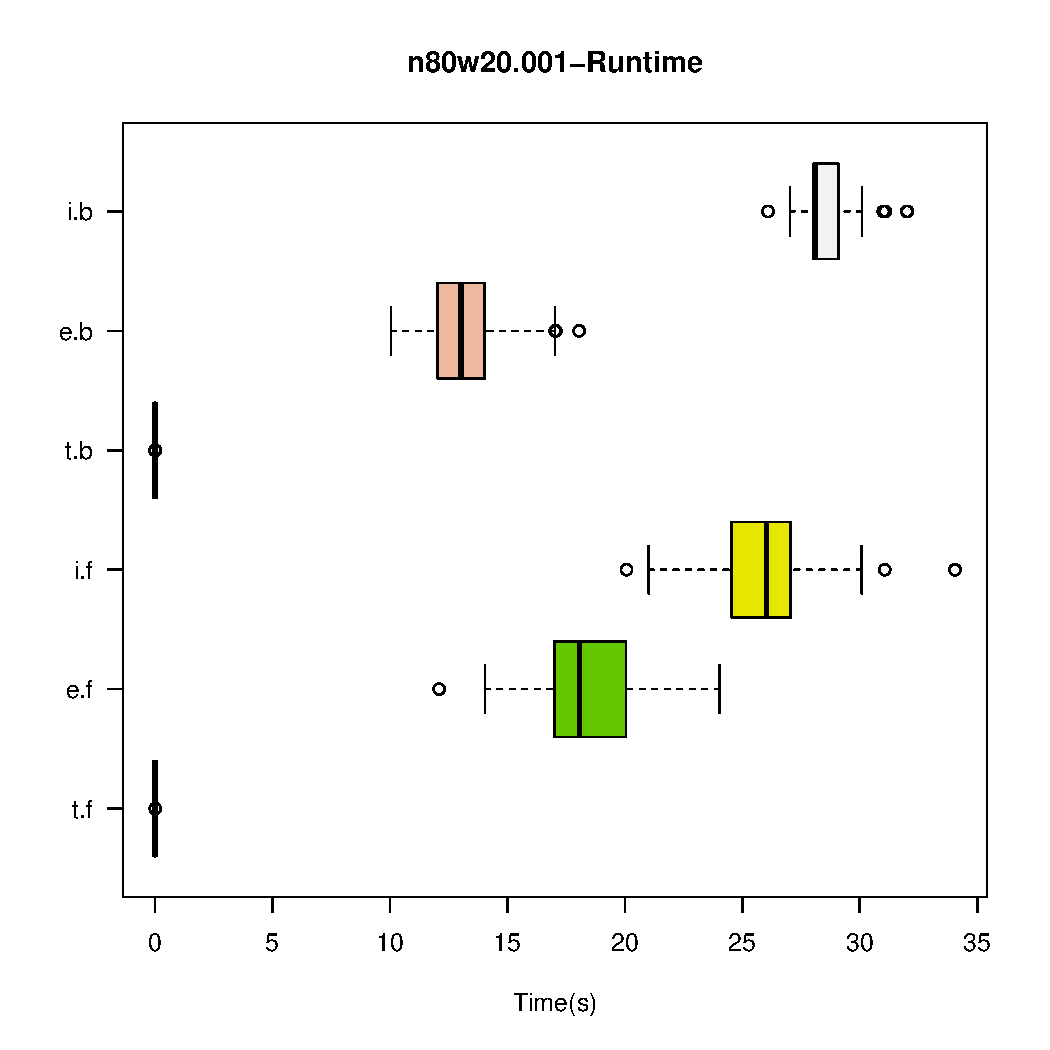
\includegraphics[width=0.6\textwidth,keepaspectratio]{{II/n80w20.001/n80w20.001-CpuTime}.pdf}
\captionof{figure}{n80w20.001 - Runtime boxplots for the different iterative improvement algorithms}
\end{center}

\begin{center}
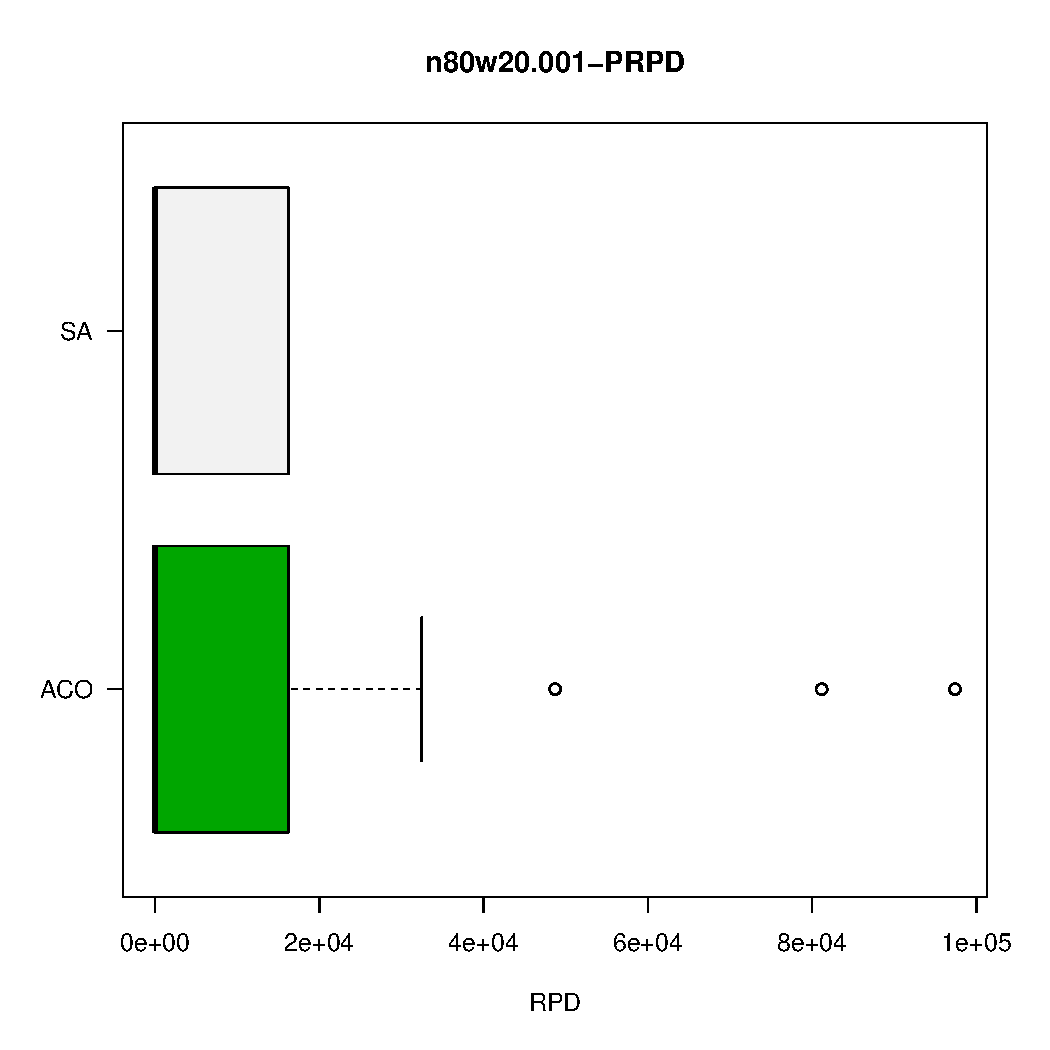
\includegraphics[width=0.6\textwidth,keepaspectratio]{{II/n80w20.001/n80w20.001-PRPD}.pdf}
\captionof{figure}{n80w20.001 - PRPD boxplots for the different iterative improvement algorithms}
\end{center}

\begin{center}
\begin{tabular}{|l|l|}
\hline
\textbf{Test} & \textbf{P-Value} \\
\hline
First vs best - Transpose&9.74631639820544e-18\\
\hline
First vs best - Exchange&2.04966732989559e-17\\
\hline
First vs best - Insert&1.74838327736385e-15\\
\hline
Exchange vs Insert - First&3.95591160889952e-18\\
\hline
Exchange vs Insert - Best&3.9556885406462e-18\\
\hline
\end{tabular}
\captionof{table}{n80w20.001 - Results of Wilcoxon paired signed rank test}
\end{center}

\subsubsection{n80w20.002}
\begin{center}
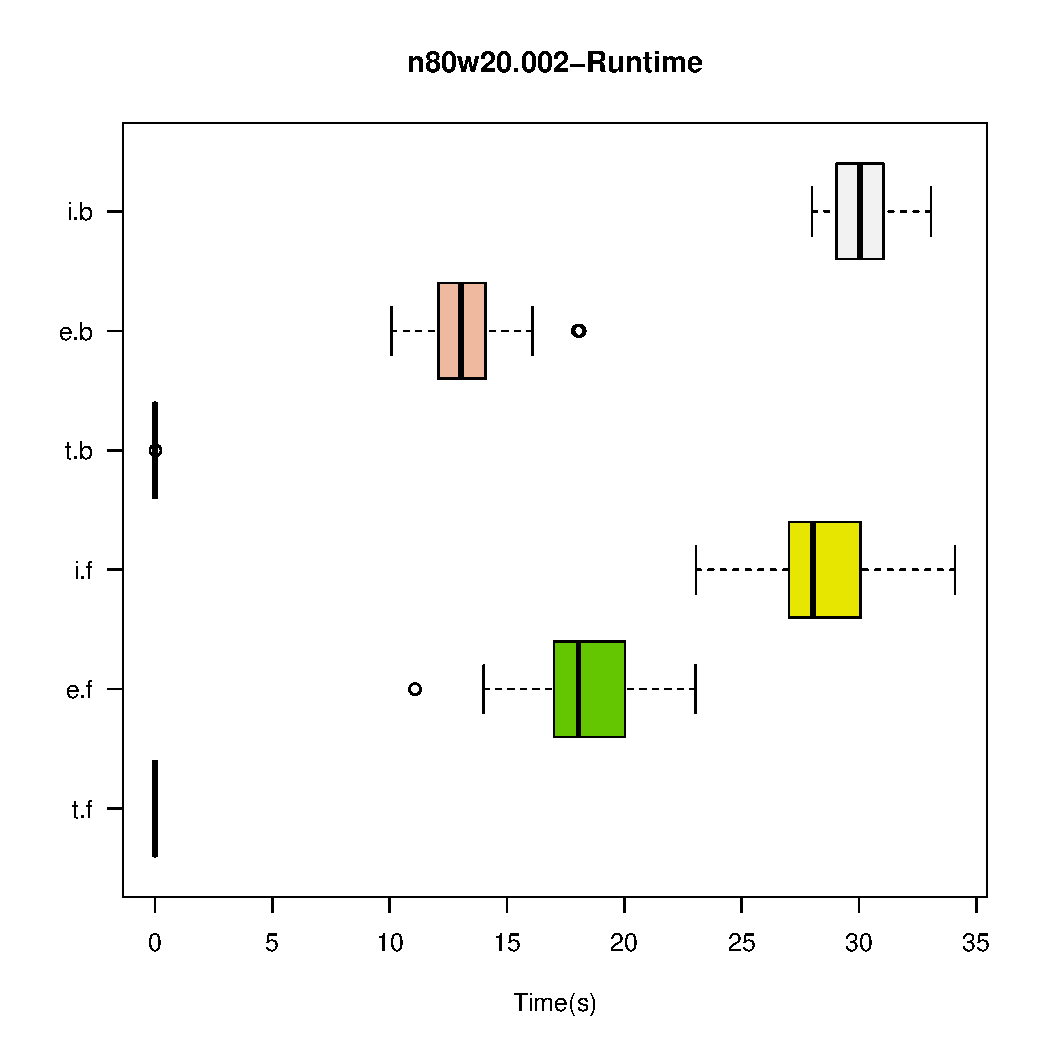
\includegraphics[width=0.6\textwidth,keepaspectratio]{{II/n80w20.002/n80w20.002-CpuTime}.pdf}
\captionof{figure}{n80w20.002 - Runtime boxplots for the different iterative improvement algorithms}
\end{center}

\begin{center}
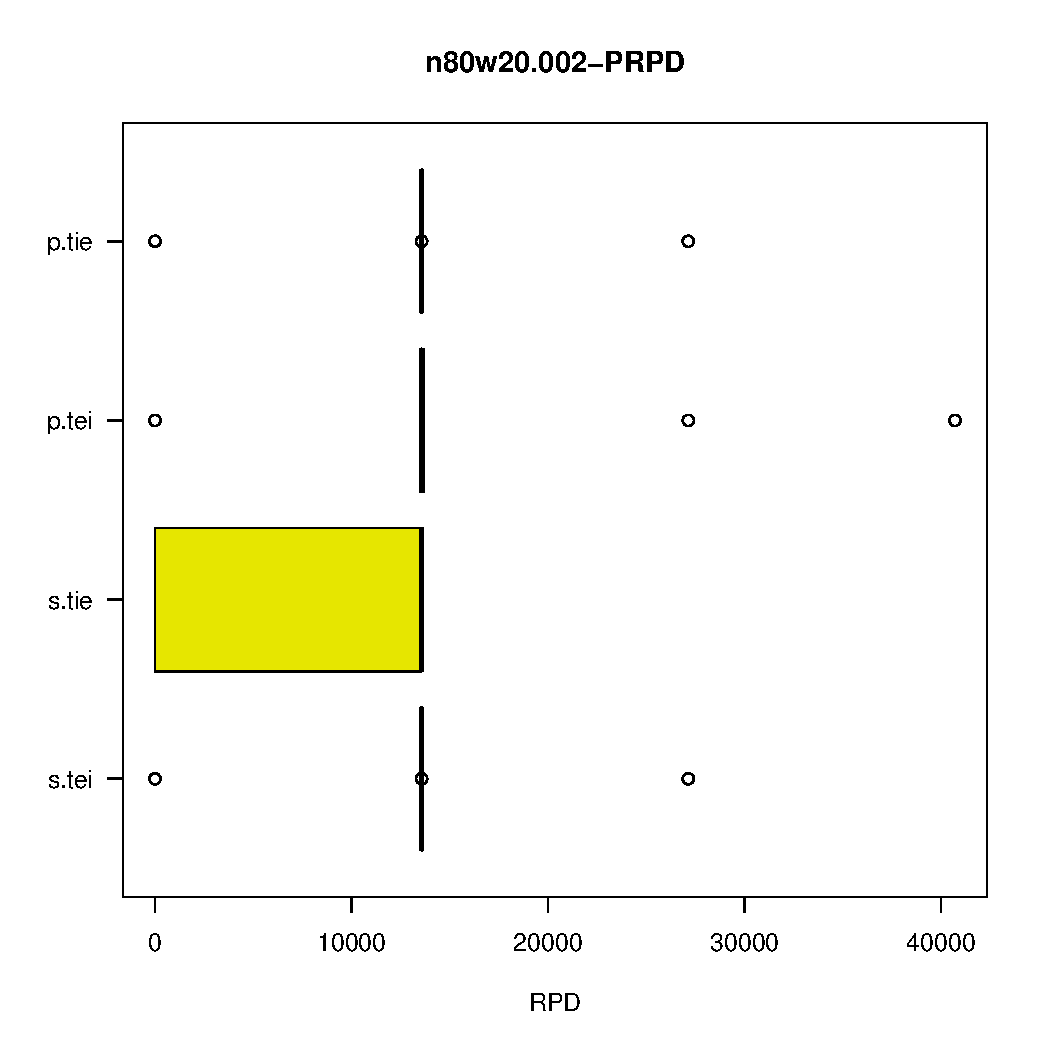
\includegraphics[width=0.6\textwidth,keepaspectratio]{{II/n80w20.002/n80w20.002-PRPD}.pdf}
\captionof{figure}{n80w20.002 - PRPD boxplots for the different iterative improvement algorithms}
\end{center}

\begin{center}
\begin{tabular}{|l|l|}
\hline
\textbf{Test} & \textbf{P-Value} \\
\hline
First vs best - Transpose&3.95591160889952e-18\\
\hline
First vs best - Exchange&1.61703099974578e-17\\
\hline
First vs best - Insert&2.39050570998277e-07\\
\hline
Exchange vs Insert - First&3.95591160889952e-18\\
\hline
Exchange vs Insert - Best&3.9556885406462e-18\\
\hline
\end{tabular}
\captionof{table}{n80w20.002 - Results of Wilcoxon paired signed rank test}
\end{center}

\subsubsection{n80w20.003}
\begin{center}
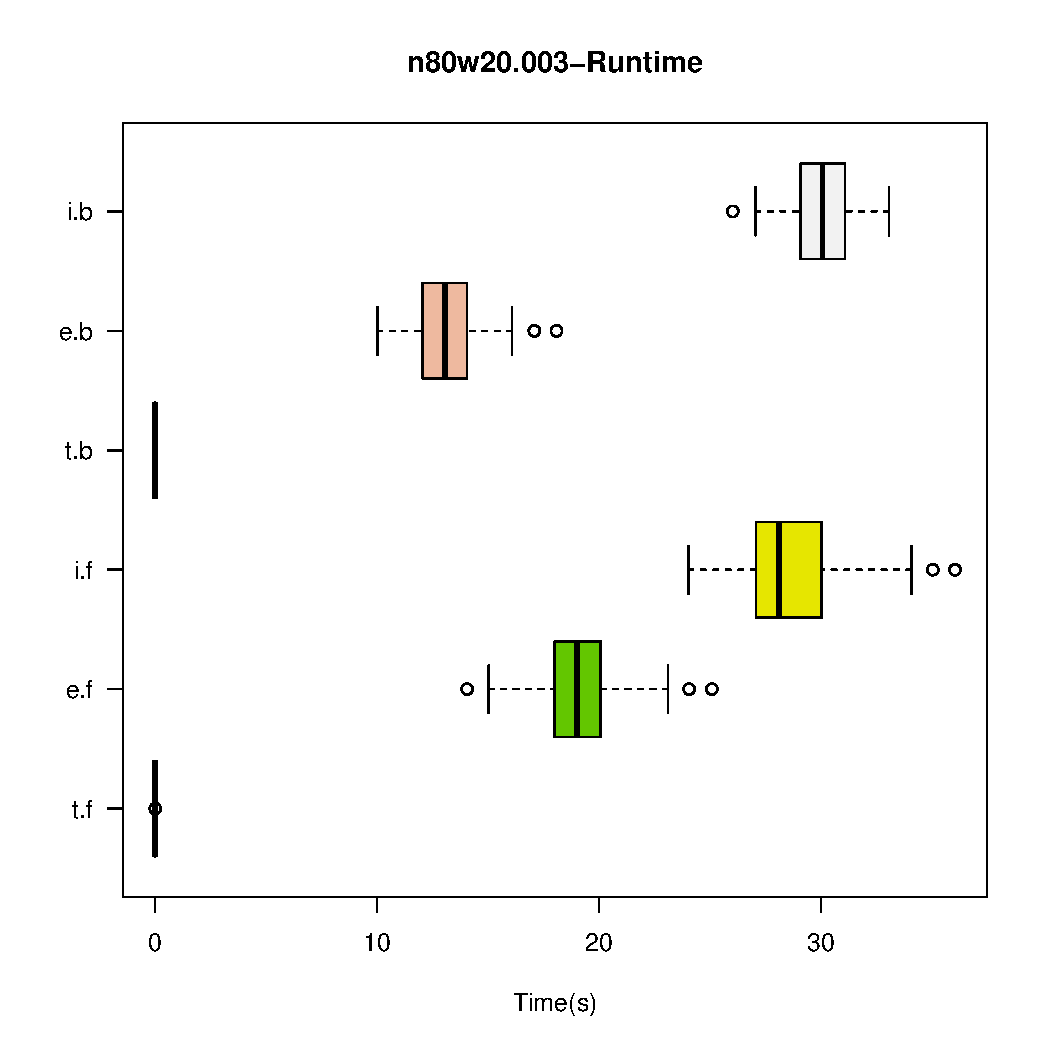
\includegraphics[width=0.6\textwidth,keepaspectratio]{{II/n80w20.003/n80w20.003-CpuTime}.pdf}
\captionof{figure}{n80w20.003 - Runtime boxplots for the different iterative improvement algorithms}
\end{center}

\begin{center}
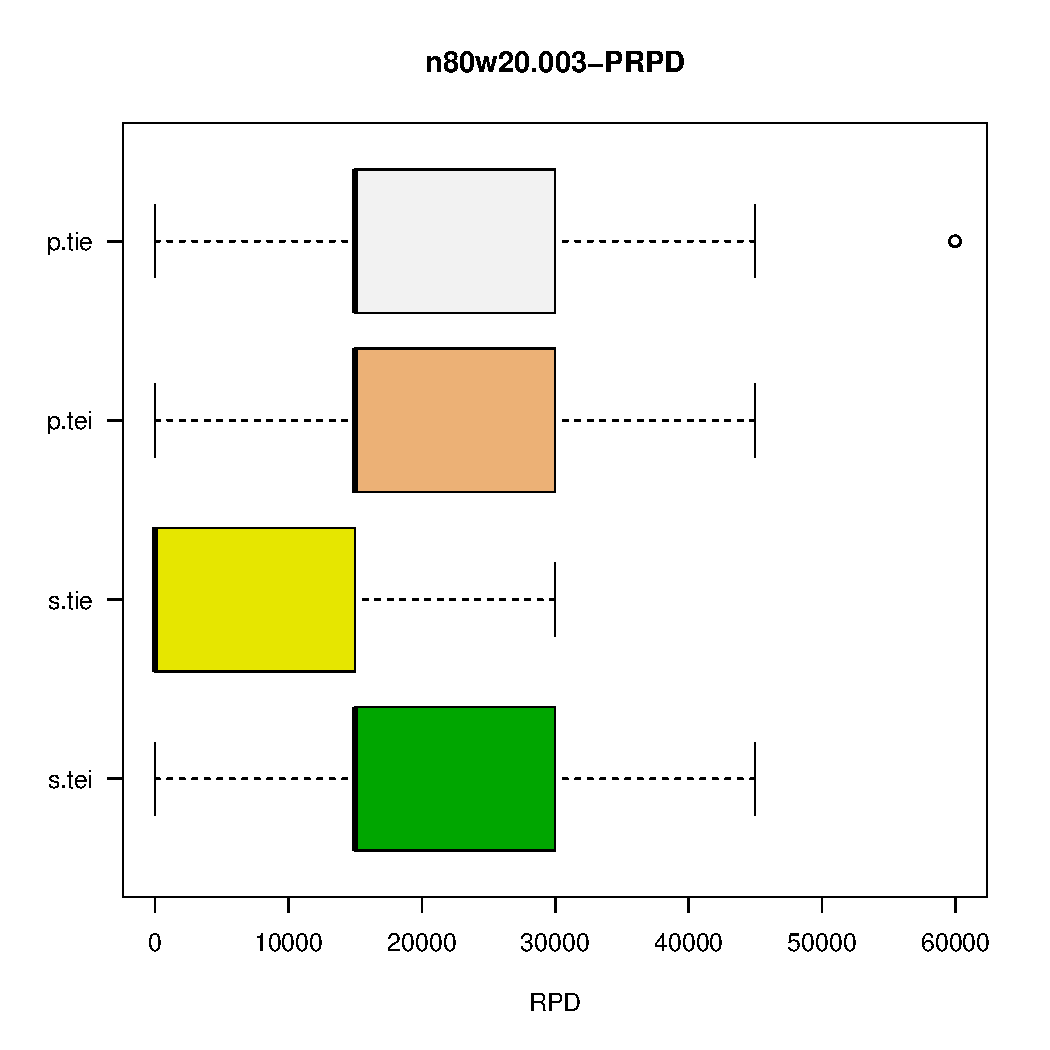
\includegraphics[width=0.6\textwidth,keepaspectratio]{{II/n80w20.003/n80w20.003-PRPD}.pdf}
\captionof{figure}{n80w20.003 - PRPD boxplots for the different iterative improvement algorithms}
\end{center}

\begin{center}
\begin{tabular}{|l|l|}
\hline
\textbf{Test} & \textbf{P-Value} \\
\hline
First vs best - Transpose&3.95591160889952e-18\\
\hline
First vs best - Exchange&6.21747363653032e-18\\
\hline
First vs best - Insert&6.2952945764779e-08\\
\hline
Exchange vs Insert - First&3.9556885406462e-18\\
\hline
Exchange vs Insert - Best&3.95591160889952e-18\\
\hline
\end{tabular}
\captionof{table}{n80w20.003 - Results of Wilcoxon paired signed rank test}
\end{center}

\subsubsection{n80w20.004}
\begin{center}
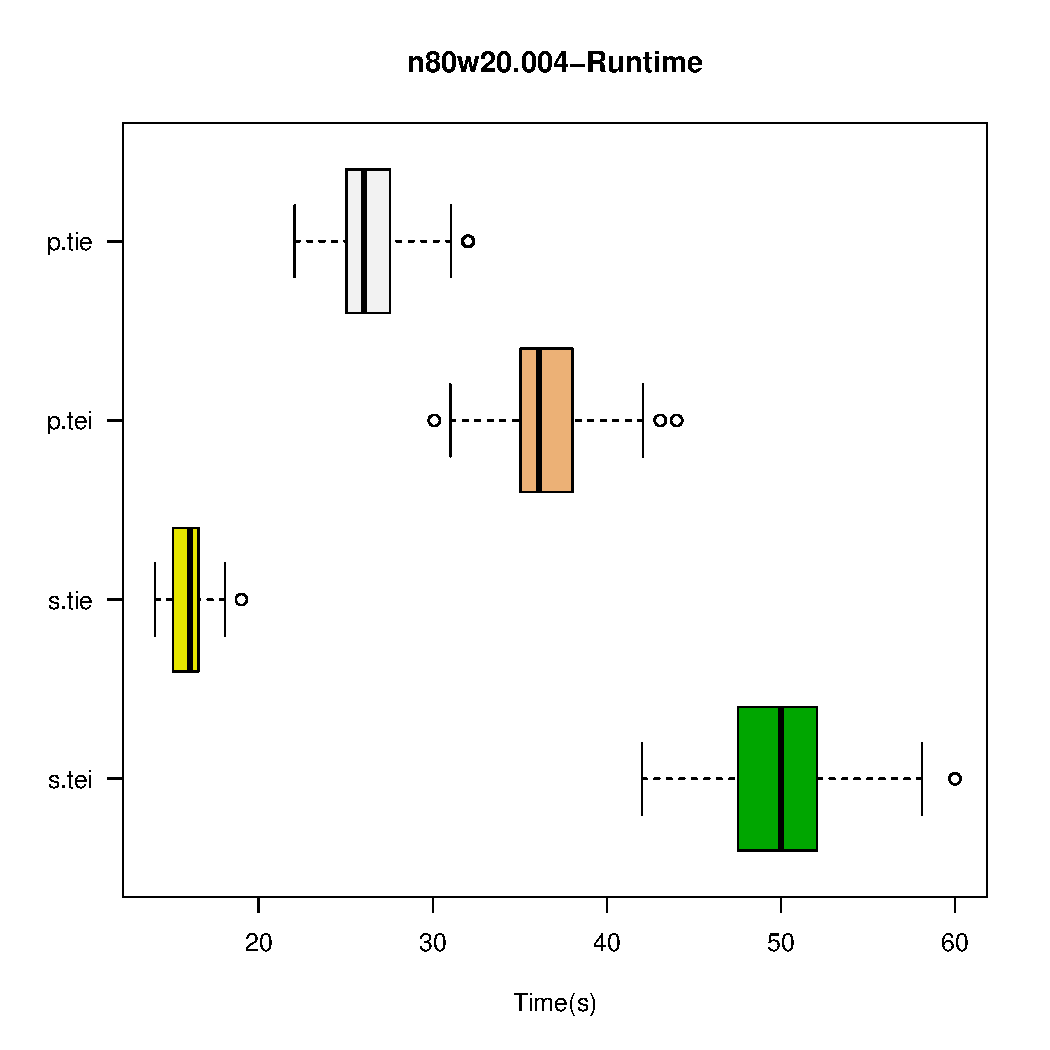
\includegraphics[width=0.6\textwidth,keepaspectratio]{{II/n80w20.004/n80w20.004-CpuTime}.pdf}
\captionof{figure}{n80w20.004 - Runtime boxplots for the different iterative improvement algorithms}
\end{center}

\begin{center}
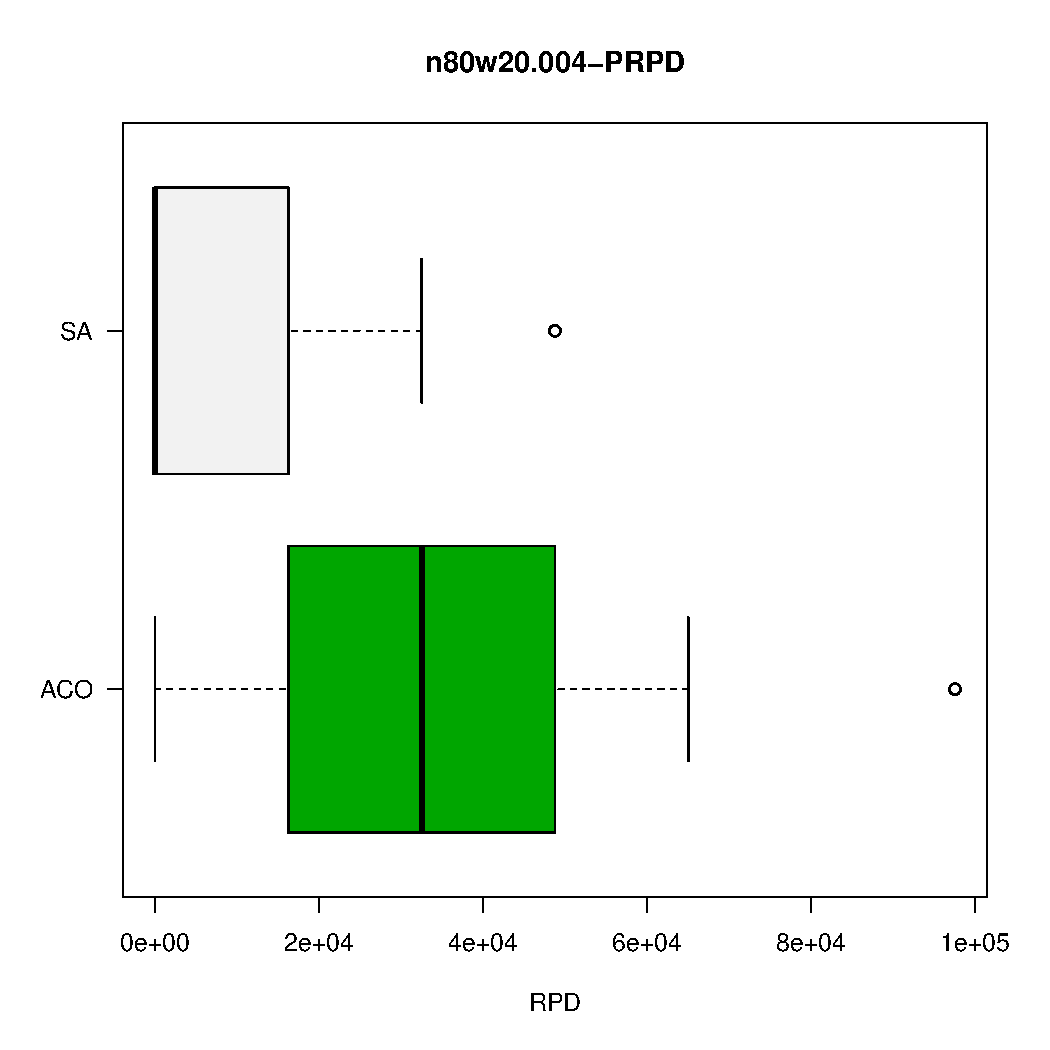
\includegraphics[width=0.6\textwidth,keepaspectratio]{{II/n80w20.004/n80w20.004-PRPD}.pdf}
\captionof{figure}{n80w20.001 - PRPD boxplots for the different iterative improvement algorithms}
\end{center}

\begin{center}
\begin{tabular}{|l|l|}
\hline
\textbf{Test} & \textbf{P-Value} \\
\hline
First vs best - Transpose&4.33123080260219e-18\\
\hline
First vs best - Exchange&1.5356610755813e-16\\
\hline
First vs best - Insert&4.27702026764362e-14\\
\hline
Exchange vs Insert - First&5.59593516960623e-18\\
\hline
Exchange vs Insert - Best&3.95591160889952e-18\\
\hline
\end{tabular}
\captionof{table}{n80w20.004 - Results of Wilcoxon paired signed rank test}
\end{center}

\subsubsection{n80w20.005}
\begin{center}
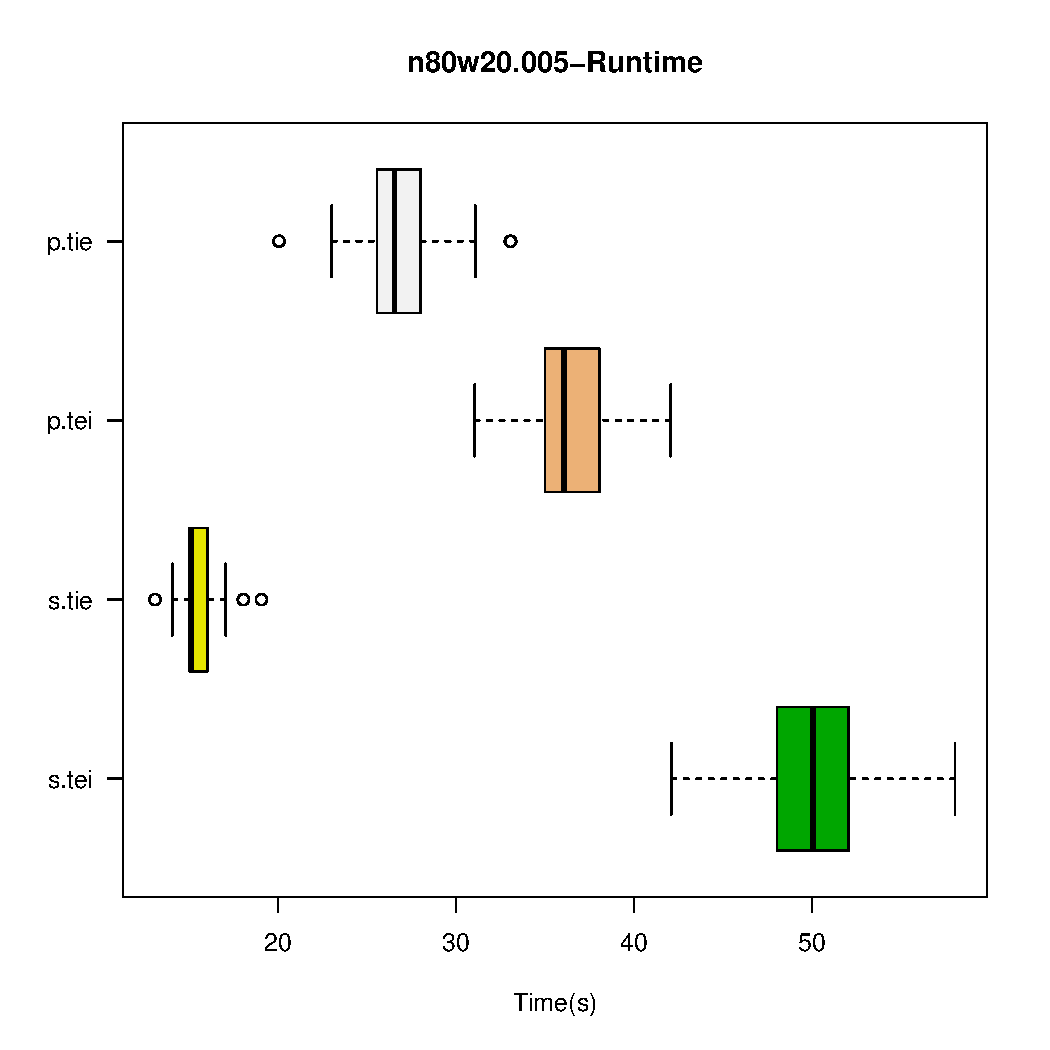
\includegraphics[width=0.6\textwidth,keepaspectratio]{{II/n80w20.005/n80w20.005-CpuTime}.pdf}
\captionof{figure}{n80w20.005 - Runtime boxplots for the different iterative improvement algorithms}
\end{center}

\begin{center}
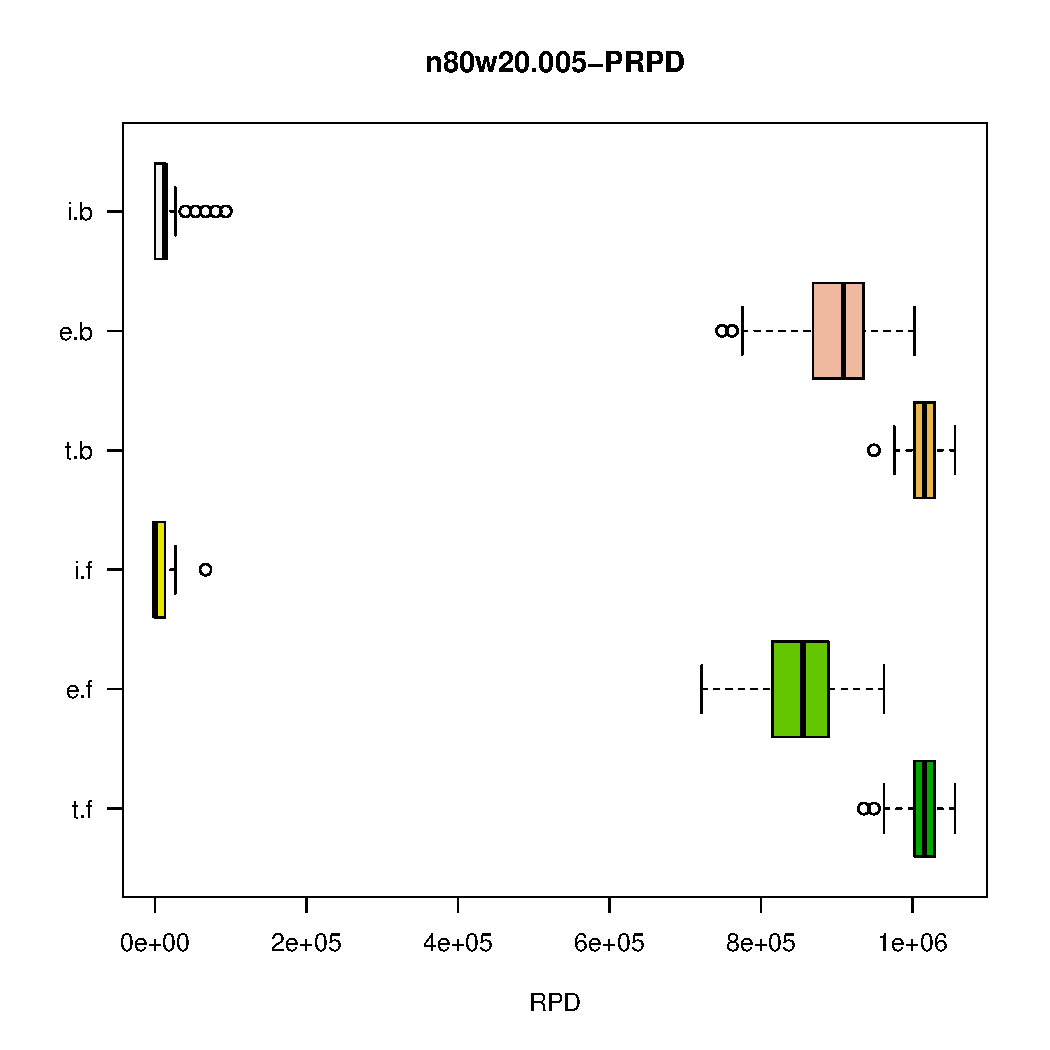
\includegraphics[width=0.6\textwidth,keepaspectratio]{{II/n80w20.005/n80w20.005-PRPD}.pdf}
\captionof{figure}{n80w20.005 - PRPD boxplots for the different iterative improvement algorithms}
\end{center}

\begin{center}
\begin{tabular}{|l|l|}
\hline
\textbf{Test} & \textbf{P-Value} \\
\hline
First vs best - Transpose&4.46398542390809e-18\\
\hline
First vs best - Exchange&4.74166029806301e-18\\
\hline
First vs best - Insert&4.0369131744045e-10\\
\hline
Exchange vs Insert - First&4.74166029806301e-18\\
\hline
Exchange vs Insert - Best&3.95591160889952e-18\\
\hline
\end{tabular}
\captionof{table}{n80w20.005 - Results of Wilcoxon paired signed rank test}
\end{center}

\subsubsection{n80w200.001}
\begin{center}
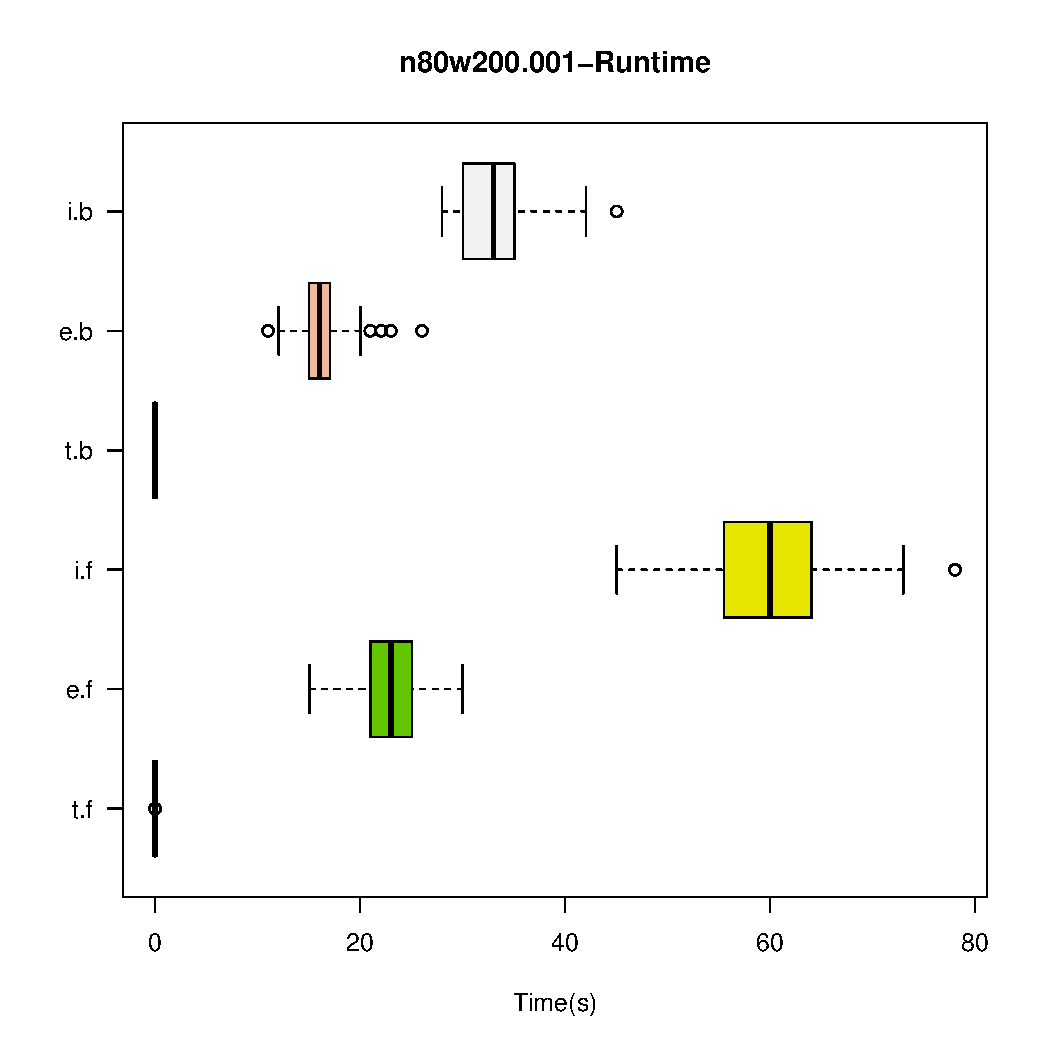
\includegraphics[width=0.6\textwidth,keepaspectratio]{{II/n80w200.001/n80w200.001-CpuTime}.pdf}
\captionof{figure}{n80w200.001 - Runtime boxplots for the different iterative improvement algorithms}
\end{center}

\begin{center}
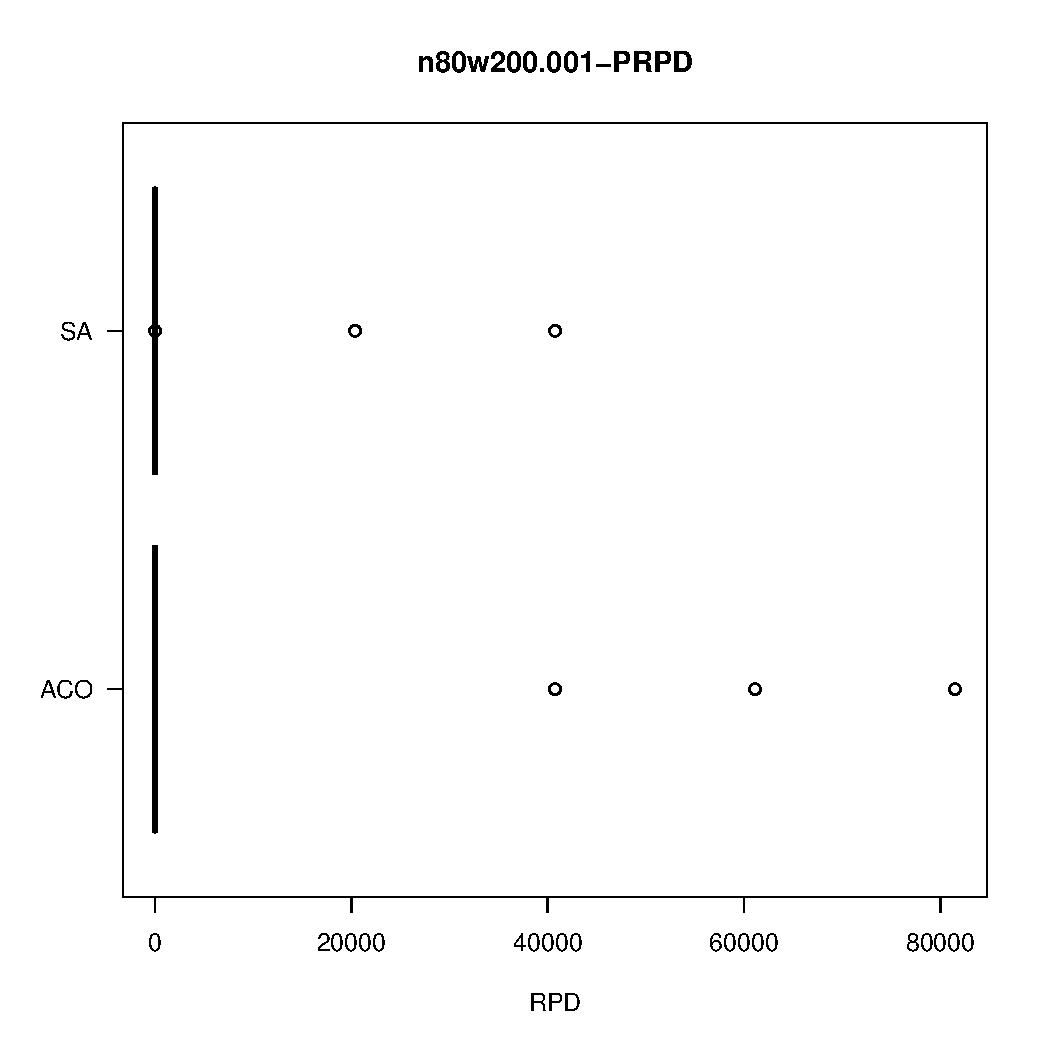
\includegraphics[width=0.6\textwidth,keepaspectratio]{{II/n80w200.001/n80w200.001-PRPD}.pdf}
\captionof{figure}{n80w200.001 - PRPD boxplots for the different iterative improvement algorithms}
\end{center}

\begin{center}
\begin{tabular}{|l|l|}
\hline
\textbf{Test} & \textbf{P-Value} \\
\hline
First vs best - Transpose&4.07730530936212e-18\\
\hline
First vs best - Exchange&2.17457280454137e-17\\
\hline
First vs best - Insert&3.95591160889952e-18\\
\hline
Exchange vs Insert - First&3.95591160889952e-18\\
\hline
Exchange vs Insert - Best&3.95591160889952e-18\\
\hline
\end{tabular}
\captionof{table}{n80w200.001 - Results of Wilcoxon paired signed rank test}
\end{center}

\subsubsection{n80w200.002}
\begin{center}
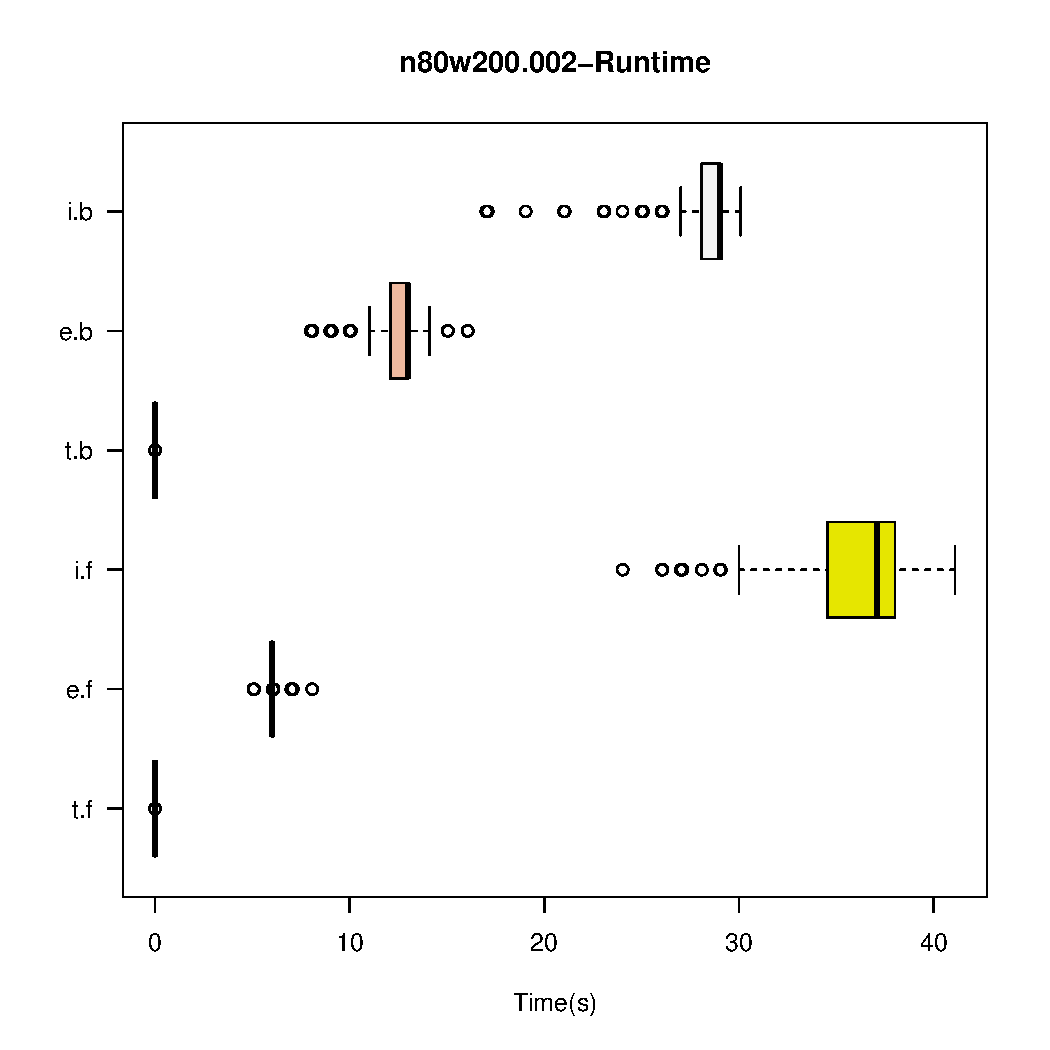
\includegraphics[width=0.6\textwidth,keepaspectratio]{{II/n80w200.002/n80w200.002-CpuTime}.pdf}
\captionof{figure}{n80w200.002 - Runtime boxplots for the different iterative improvement algorithms}
\end{center}

\begin{center}
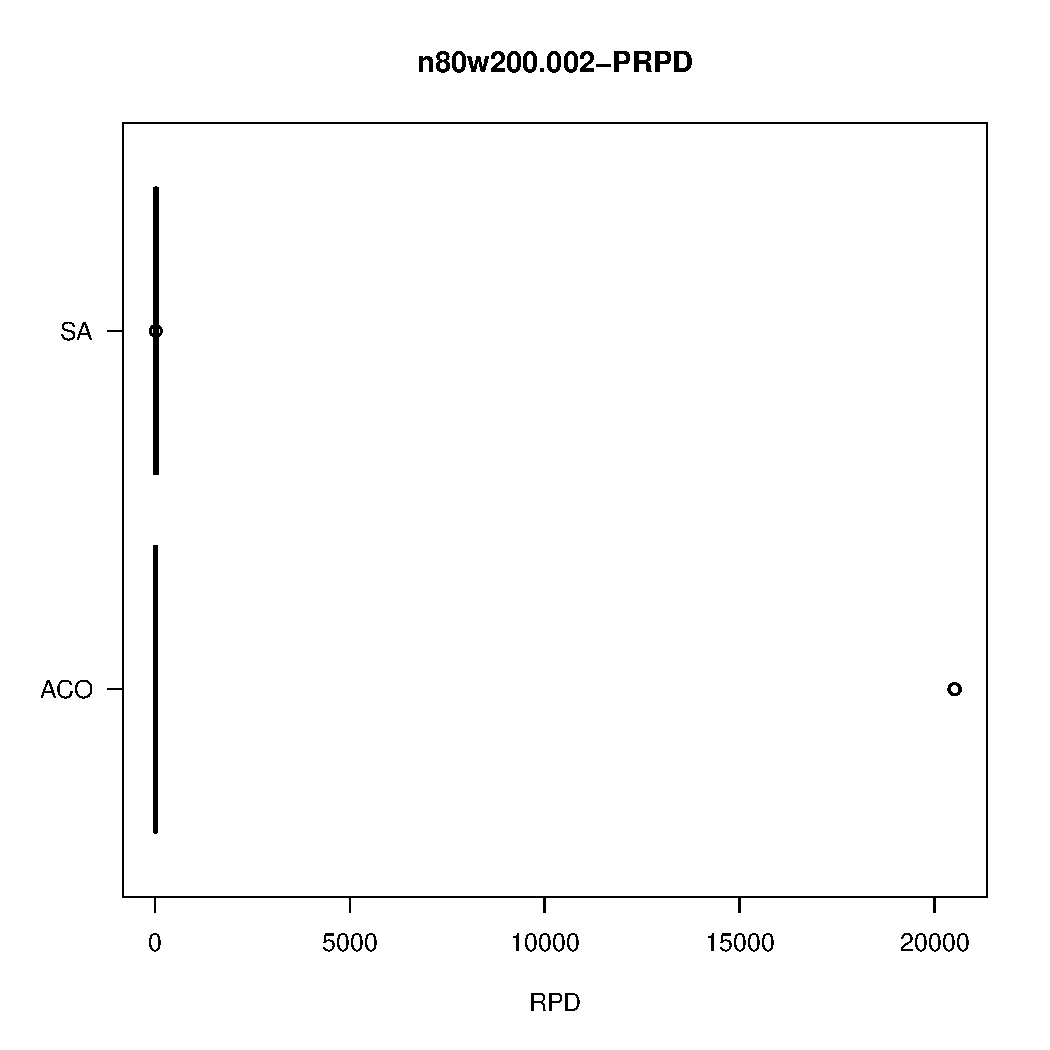
\includegraphics[width=0.6\textwidth,keepaspectratio]{{II/n80w200.002/n80w200.002-PRPD}.pdf}
\captionof{figure}{n80w200.002 - PRPD boxplots for the different iterative improvement algorithms}
\end{center}

\begin{center}
\begin{tabular}{|l|l|}
\hline
\textbf{Test} & \textbf{P-Value} \\
\hline
First vs best - Transpose&5.19043683699158e-18\\
\hline
First vs best - Exchange&4.6720416035814e-17\\
\hline
First vs best - Insert&3.95591160889952e-18\\
\hline
Exchange vs Insert - First&3.95591160889952e-18\\
\hline
Exchange vs Insert - Best&3.95591160889952e-18\\
\hline
\end{tabular}
\captionof{table}{n80w200.002 - Results of Wilcoxon paired signed rank test}
\end{center}

\subsubsection{n80w200.003}
\begin{center}
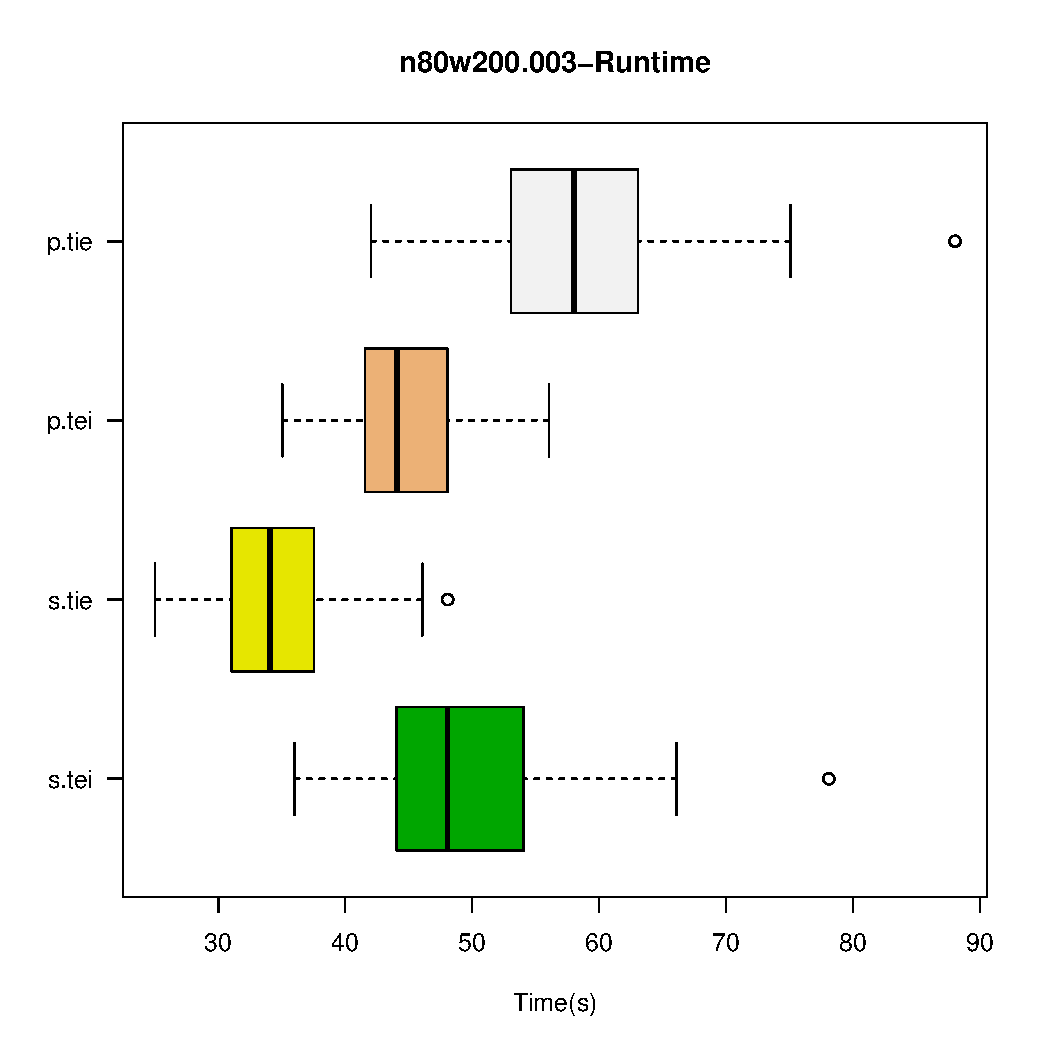
\includegraphics[width=0.6\textwidth,keepaspectratio]{{II/n80w200.003/n80w200.003-CpuTime}.pdf}
\captionof{figure}{n80w200.003 - Runtime boxplots for the different iterative improvement algorithms}
\end{center}

\begin{center}
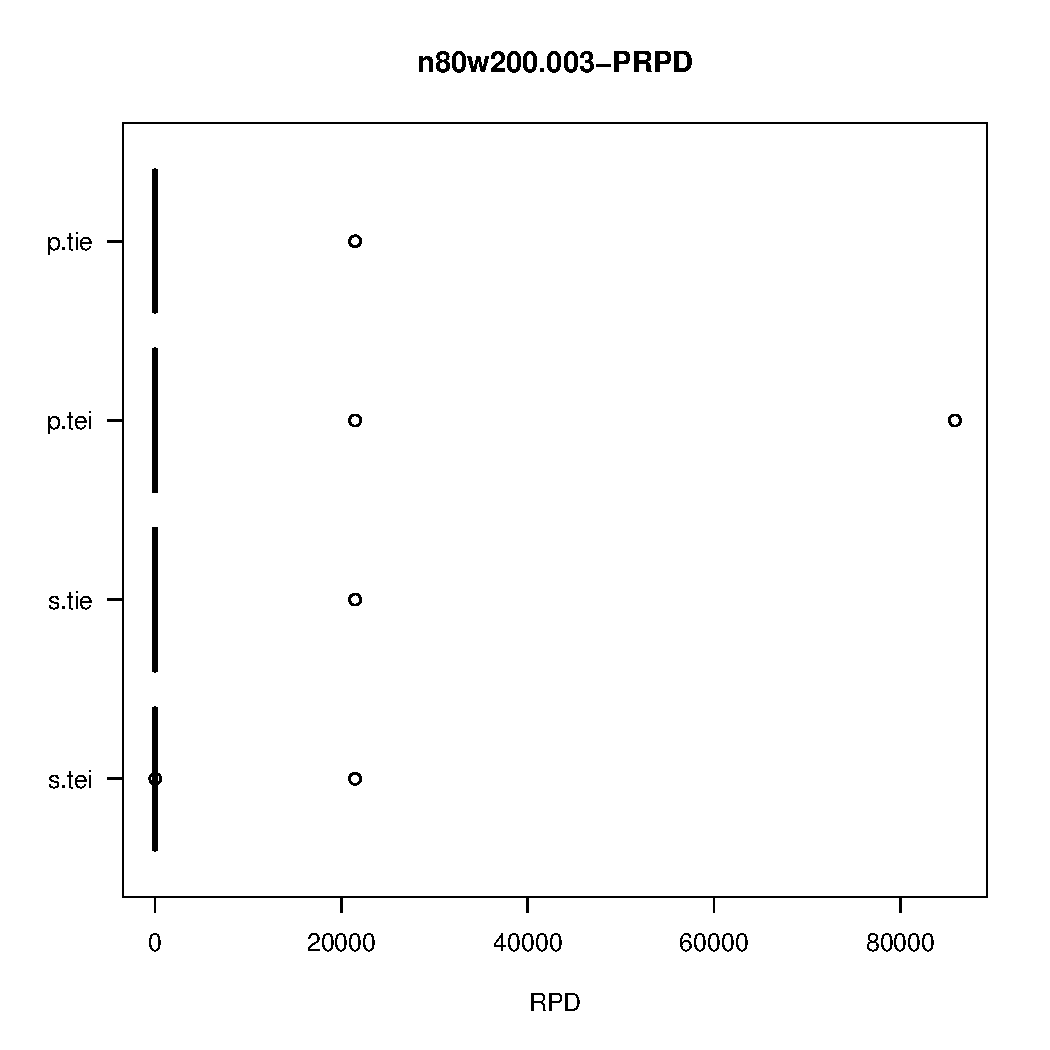
\includegraphics[width=0.6\textwidth,keepaspectratio]{{II/n80w200.003/n80w200.003-PRPD}.pdf}
\captionof{figure}{n80w200.003 - PRPD boxplots for the different iterative improvement algorithms}
\end{center}

\begin{center}
\begin{tabular}{|l|l|}
\hline
\textbf{Test} & \textbf{P-Value} \\
\hline
First vs best - Transpose&4.33123080260219e-18\\
\hline
First vs best - Exchange&7.01070639830382e-18\\
\hline
First vs best - Insert&3.95591160889952e-18\\
\hline
Exchange vs Insert - First&3.95591160889952e-18\\
\hline
Exchange vs Insert - Best&3.95591160889952e-18\\
\hline
\end{tabular}
\captionof{table}{n80w200.003 - Results of Wilcoxon paired signed rank test}
\end{center}

\subsubsection{n80w200.004}
\begin{center}
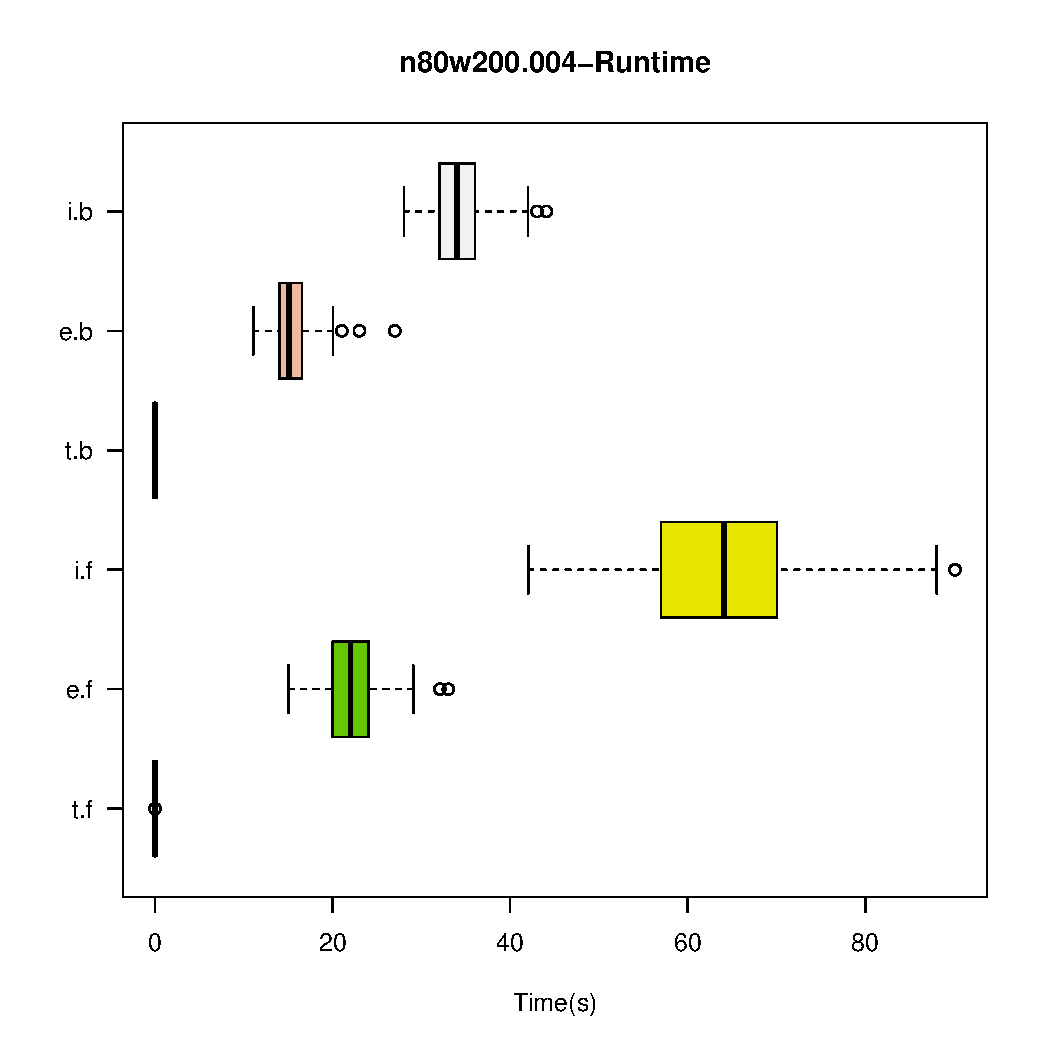
\includegraphics[width=0.6\textwidth,keepaspectratio]{{II/n80w200.004/n80w200.004-CpuTime}.pdf}
\captionof{figure}{n80w200.004 - Runtime boxplots for the different iterative improvement algorithms}
\end{center}

\begin{center}
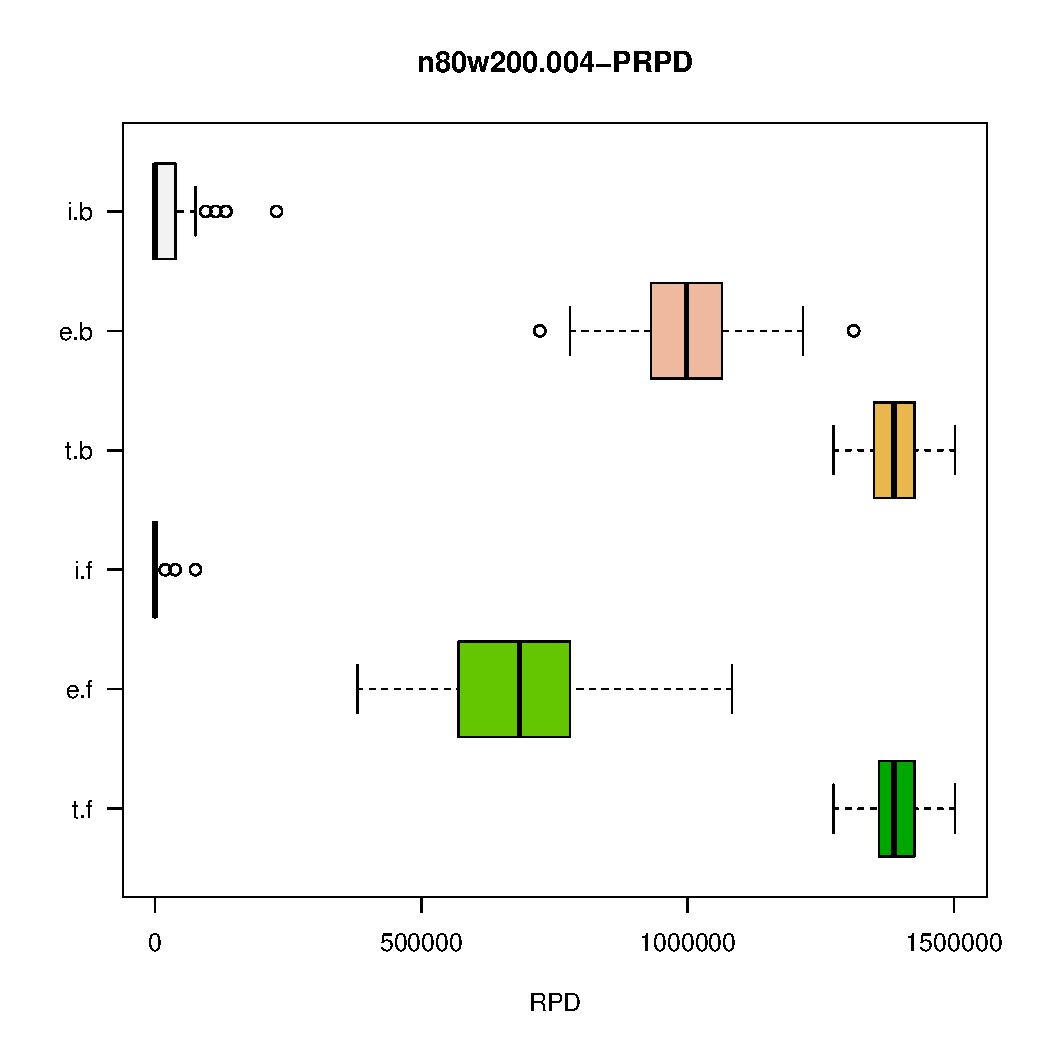
\includegraphics[width=0.6\textwidth,keepaspectratio]{{II/n80w200.004/n80w200.004-PRPD}.pdf}
\captionof{figure}{n80w200.001 - PRPD boxplots for the different iterative improvement algorithms}
\end{center}

\begin{center}
\begin{tabular}{|l|l|}
\hline
\textbf{Test} & \textbf{P-Value} \\
\hline
First vs best - Transpose&4.33123080260219e-18\\
\hline
First vs best - Exchange&2.4473398426105e-17\\
\hline
First vs best - Insert&3.95591160889952e-18\\
\hline
Exchange vs Insert - First&3.95591160889952e-18\\
\hline
Exchange vs Insert - Best&3.95591160889952e-18\\
\hline
\end{tabular}
\captionof{table}{n80w200.004 - Results of Wilcoxon paired signed rank test}
\end{center}

\subsubsection{n80w200.005}
\begin{center}
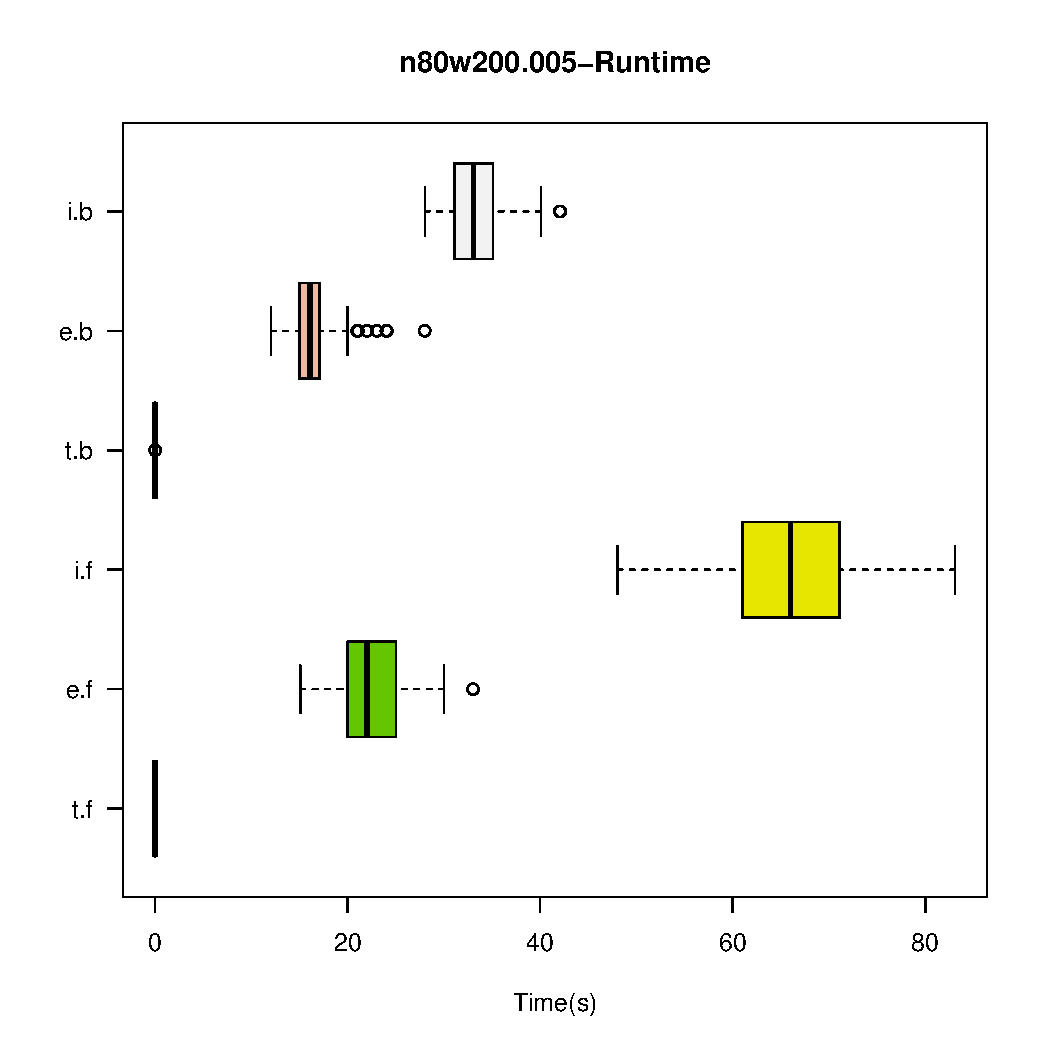
\includegraphics[width=0.6\textwidth,keepaspectratio]{{II/n80w200.005/n80w200.005-CpuTime}.pdf}
\captionof{figure}{n80w200.005 - Runtime boxplots for the different iterative improvement algorithms}
\end{center}

\begin{center}
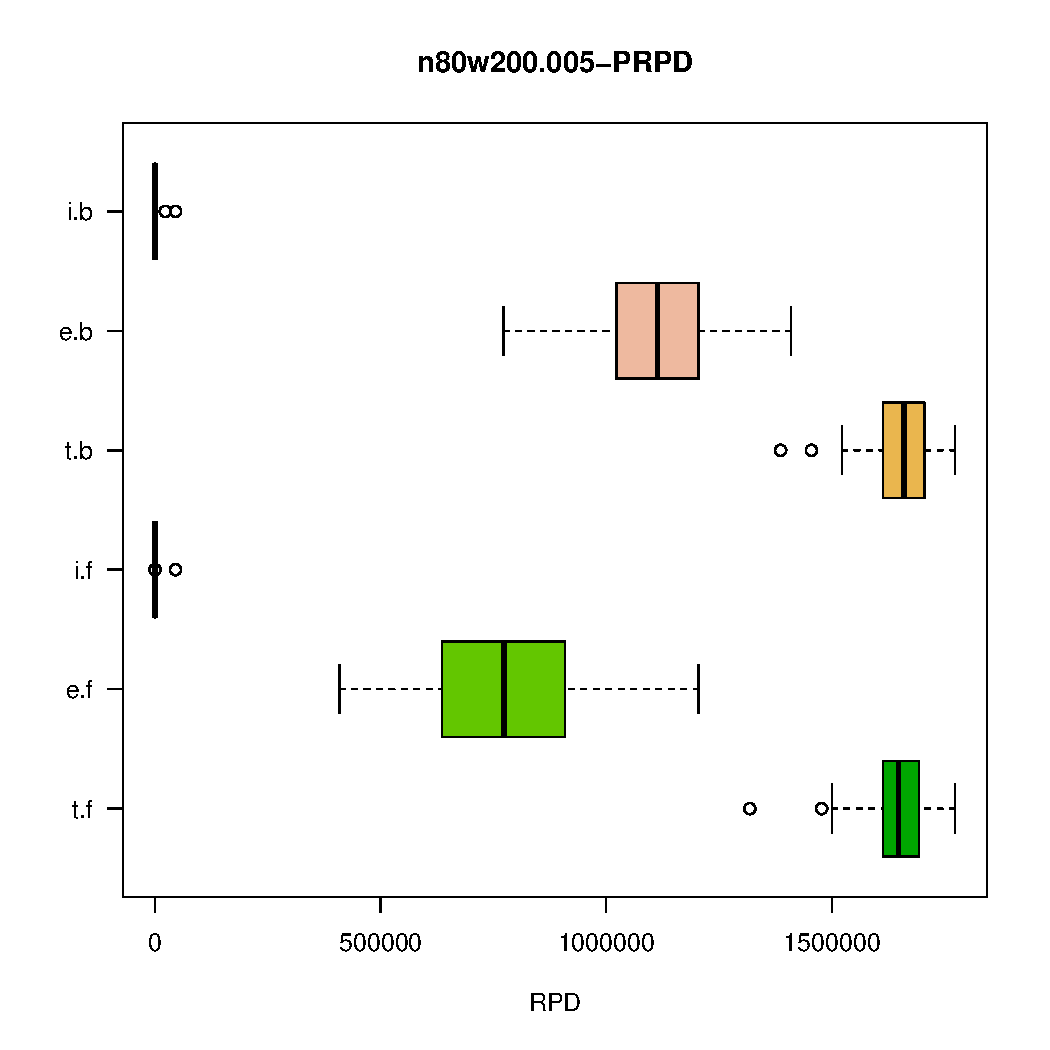
\includegraphics[width=0.6\textwidth,keepaspectratio]{{II/n80w200.005/n80w200.005-PRPD}.pdf}
\captionof{figure}{n80w200.005 - PRPD boxplots for the different iterative improvement algorithms}
\end{center}

\begin{center}
\begin{tabular}{|l|l|}
\hline
\textbf{Test} & \textbf{P-Value} \\
\hline
First vs best - Transpose&4.74166029806301e-18\\
\hline
First vs best - Exchange&1.40854365025687e-16\\
\hline
First vs best - Insert&3.95591160889952e-18\\
\hline
Exchange vs Insert - First&3.95591160889952e-18\\
\hline
Exchange vs Insert - Best&3.95591160889952e-18\\
\hline
\end{tabular}
\captionof{table}{n80w200.005 - Results of Wilcoxon paired signed rank test}
\end{center}

\subsection{Statistics}

\subsubsection{Transpose-First Improvement}
\begin{center}
\begin{tabular}{|l|c|l|l|}
\hline
\textbf{Instance}& \textbf{\% Infeasible} & $\mathbf{\bar{PRDP}}$ &$\mathbf{\bar{Runtime}}$\\
\hline
n80w20.001&1&1229712.6&0.0100035563\\
\hline
n80w20.002&1&1028075.17&0.0095843375\\
\hline
n80w20.003&1&1132968.5&0.0098099452\\
\hline
n80w20.005&1&1010681.79&0.0097989762\\
\hline
n80w20.004&1&1226174.6&0.0094877067\\
\hline
n80w200.001&1&1467634.1&0.0098152878\\
\hline
n80w200.002&1&1504523.7&0.0099101404\\
\hline
n80w200.004&1&1388037.6&0.0098893615\\
\hline
n80w200.003&1&1567210.5&0.0097697727\\
\hline
n80w200.005&1&1644110.9&0.0097550971\\
\hline
\end{tabular}
\captionof{table}{Statistics summary for iterative improvement algorithm with Transpose neighborhood and First Improvement pivoting rule}
\end{center}

\subsubsection{Transpose-Best Improvement}
\begin{center}
\begin{tabular}{|l|c|l|l|}
\hline
\textbf{Instance}& \textbf{\% Infeasible} & $\mathbf{\bar{PRDP}}$ &$\mathbf{\bar{Runtime}}$\\
\hline
n80w20.001&1&1236039.3&0.014545497\\
\hline
n80w20.002&1&1033090.48&0.0145450422\\
\hline
n80w20.003&1&1137758.7&0.014536776\\
\hline
n80w20.005&1&1014818.46&0.014947609\\
\hline
n80w20.004&1&1232996&0.015151286\\
\hline
n80w200.001&1&1476994.8&0.0147534638\\
\hline
n80w200.002&1&1511281&0.014884921\\
\hline
n80w200.004&1&1392023.3&0.0146445173\\
\hline
n80w200.003&1&1575355.5&0.0143582468\\
\hline
n80w200.005&1&1653419.6&0.0150098656\\
\hline
\end{tabular}
\captionof{table}{Statistics summary for iterative improvement algorithm with Transpose neighborhood and Best Improvement pivoting rule}
\end{center}

\subsubsection{Exchange-First Improvement}
\begin{center}
\begin{tabular}{|l|c|l|l|}
\hline
\textbf{Instance}& \textbf{\% Infeasible} & $\mathbf{\bar{PRDP}}$ &$\mathbf{\bar{Runtime}}$\\
\hline
n80w20.001&1&1035718.78&18.390814\\
\hline
n80w20.002&1&884386.3&18.198632\\
\hline
n80w20.003&1&956518.77&18.913801\\
\hline
n80w20.005&1&849054.52&19.043496\\
\hline
n80w20.004&1&1030411.56&19.660314\\
\hline
n80w200.001&1&661322.18&23.117446\\
\hline
n80w200.002&1&813339.6&22.552976\\
\hline
n80w200.004&1&679489.06&22.068859\\
\hline
n80w200.003&1&697450.03&24.338257\\
\hline
n80w200.005&1&760027.65&22.348975\\
\hline
\end{tabular}
\captionof{table}{Statistics summary for iterative improvement algorithm with Exchange neighborhood and First Improvement pivoting rule}
\end{center}

\subsubsection{Exchange-Best Improvement}
\begin{center}
\begin{tabular}{|l|c|l|l|}
\hline
\textbf{Instance}& \textbf{\% Infeasible} & $\mathbf{\bar{PRDP}}$ &$\mathbf{\bar{Runtime}}$\\
\hline
n80w20.001&1&1086217.68&13.091453\\
\hline
n80w20.002&1&901762.05&13.365301\\
\hline
n80w20.003&1&1017243.86&13.267128\\
\hline
n80w20.005&1&895720.53&13.5824245\\
\hline
n80w20.004&1&1084080.4&14.189582\\
\hline
n80w200.001&1&1022433.76&16.418229\\
\hline
n80w200.002&1&1075649.94&16.028712\\
\hline
n80w200.004&1&994703.67&15.518766\\
\hline
n80w200.003&1&1094460.9&16.16696\\
\hline
n80w200.005&1&1110949.86&16.566802\\
\hline
\end{tabular}
\captionof{table}{Statistics summary for iterative improvement algorithm with Exchange neighborhood and Best Improvement pivoting rule}
\end{center}

\subsubsection{Insert-First Improvement}
\begin{center}
\begin{tabular}{|l|c|l|l|}
\hline
\textbf{Instance}& \textbf{\% Infeasible} & $\mathbf{\bar{PRDP}}$ &$\mathbf{\bar{Runtime}}$\\
\hline
n80w20.001&0.65&16070.27322082&25.88279\\
\hline
n80w20.002&0.83&11803.71462682&28.509938\\
\hline
n80w20.003&0.83&21587.617&28.579453\\
\hline
n80w20.005&0.32&4945.642107&28.672083\\
\hline
n80w20.004&0.49&10894.01867489&28.474429\\
\hline
n80w200.001&0.22&6119.9927045&59.544212\\
\hline
n80w200.002&0&11.2561521&64.580306\\
\hline
n80w200.004&0.11&3049.80805246&63.942238\\
\hline
n80w200.003&0.01&437.87774695&63.687806\\
\hline
n80w200.005&0.01&464.62990671&66.084369\\
\hline

\end{tabular}
\captionof{table}{Statistics summary for iterative improvement algorithm with Insert neighborhood and First Improvement pivoting rule}
\end{center}

\subsubsection{Insert-Best Improvement}
\begin{center}
\begin{tabular}{|l|c|l|l|}
\hline
\textbf{Instance}& \textbf{\% Infeasible} & $\mathbf{\bar{PRDP}}$ &$\mathbf{\bar{Runtime}}$\\
\hline
n80w20.001&0.56&14772.44442862&28.769951\\
\hline
n80w20.002&0.84&16009.51797952&30.159812\\
\hline
n80w20.003&0.89&26984.256&30.197019\\
\hline
n80w20.005&0.52&10159.3062354&30.776906\\
\hline
n80w20.004&0.59&18861.32619536&31.013\\
\hline
n80w200.001&0.37&21195.2243605&33.031965\\
\hline
n80w200.002&0&13.2172159&33.011011\\
\hline
n80w200.004&0.42&23019.4946845&34.123681\\
\hline
n80w200.003&0.12&7740.06242146&34.080592\\
\hline
n80w200.005&0.07&2516.0079072&33.450537\\
\hline
\end{tabular}
\captionof{table}{Statistics summary for iterative improvement algorithm with Insert neighborhood and Best Improvement pivoting rule}
\end{center}

\end{homeworkProblem}		
